%% ****** Start of file apstemplate.tex ****** %
%%
%% This file is part of the APS files in the REVTeX 4 distribution.
%% Version 4.1r of REVTeX, August 2010
%%
%%
%% Copyright (c) 2001, 2009, 2010 The American Physical Society.
%%
%% See the REVTeX 4 README file for restrictions and more information.
%%
%
% This is a template for producing manuscripts for use with REVTEX 4.0
% Copy this file to another name and then work on that file.
% That way, you always have this original template file to use.
%
% Group addresses by affiliation; use superscriptaddress for long
% author lists, or if there are many overlapping affiliations.
% For Phys. Rev. appearance, change preprint to twocolumn.
% Choose pra, prb, prc, prd, pre, prl, prstab, prstper, or rmp for journal
%  Add 'draft' option to mark overfull boxes with black boxes
%  Add 'showpacs' option to make PACS codes appear
%  Add 'showkeys' option to make keywords appear
\documentclass[aps,pra,reprint,longbibliography,groupedaddress]{revtex4-1}
%\documentclass[aps,prl,preprint,superscriptaddress]{revtex4-1}
%\documentclass[aps,prl,reprint,groupedaddress]{revtex4-1}

% You should use BibTeX and apsrev.bst for references
% Choosing a journal automatically selects the correct APS
% BibTeX style file (bst file), so only uncomment the line
% below if necessary.
%\bibliographystyle{apsrev4-1}
\usepackage{graphicx}
\usepackage{amssymb, amsmath}
\usepackage{esdiff} % use this package for derivative and partial derivate commands of \diff{}{} and \diffp{}{}
\usepackage{siunitx}
\usepackage{multirow}
\usepackage{verbatim}
\usepackage{newfloat}
\usepackage{afterpage} 
\usepackage{xr}
\DeclareSIUnit\cells{cells}
\DeclareMathOperator{\hilbert}{\mathcal{H}} % To define additional named operators
\DeclareMathOperator{\h}{h} % To define additional named operators
\DeclareMathOperator{\unwrap}{unwrap} % To define additional named operators
\DeclareMathOperator{\vercat}{cat_\downarrow} % To define additional named operators
\DeclareMathOperator{\horcat}{cat_\rightarrow} % To define additional named operators
\DeclareFloatingEnvironment[name={Supplementary Figure}]{suppfigure}
\renewcommand{\thefigure}{S\arabic{figure}}
\renewcommand{\thetable}{S\arabic{table}}
\externaldocument[M-]{main}



\begin{document}

% Use the \preprint command to place your local institutional report
% number in the upper righthand corner of the title page in preprint mode.
% Multiple \preprint commands are allowed.
% Use the 'preprintnumbers' class option to override journal defaults
% to display numbers if necessary
%\preprint{}

%Title of paper
\title{High-throughput label-free cell classification using machine learning}

% repeat the \author .. \affiliation  etc. as needed
% \email, \thanks, \homepage, \altaffiliation all apply to the current
% author. Explanatory text should go in the []'s, actual e-mail
% address or url should go in the {}'s for \email and \homepage.
% Please use the appropriate macro foreach each type of information

% \affiliation command applies to all authors since the last
% \affiliation command. The \affiliation command should follow the
% other information
% \affiliation can be followed by \email, \homepage, \thanks as well.
\author{Claire L. Chen}
%\homepage[]{Your web page}
%\thanks{}
\author{Ata Mahjoubfar}
\author{Li-Chia Tai}
\author{Ian K. Blaby}
\author{Allen Huang}
\author{Kayvan R. Niazi}
\author{Bahram Jalali}

%Collaboration name if desired (requires use of superscriptaddress
%option in \documentclass). \noaffiliation is required (may also be
%used with the \author command).
%\collaboration can be followed by \email, \homepage, \thanks as well.
%\collaboration{}
%\noaffiliation

\date{\today}


% insert suggested PACS numbers in braces on next line
%\pacs{}
% insert suggested keywords - APS authors don't need to do this

%\maketitle must follow title, authors, abstract, \pacs, and \keywords
\maketitle

% body of paper here - Use proper section commands
% References should be done using the \cite, \ref, and \label commands
\section*{Supplementary methods}

\section{PCA}
[]PCA
To speed up the computation for high dimensionality analysis, we employ PCA. We have performed PCA on the 16 dimensional data set acquired by our time stretch QPI system. This maps the data from the physical feature space to the PCA space. Fig.~\ref{fig:PCA} shows the percent of the variance in data explained by each component (lower chart). The key observation is that most of the variance can be accounted for by the first two principle components. The upper portion of the plot shows the AUC for binary classification using each of the principle components. Interestingly, the first component with the highest explained variance is not necessarily the most important component for classification. This is not surprising since PCA components are optimized to the variance of data but not to the data labels. Therefore, apriori intuition about the physical significance of the features in the case here, is superior to PCA in eliminating dimensions that do not provide high value in classification. Nevertheless, in situations where physical intuition about meaning of features does not exist, PCA is a valuable tool. A second observation is that principle components that have low explained variance do have some value in classification. By revealing the structure in data that best explains the variance, PCA achieves data compression via dimensionality reduction.

[]
As shown in Fig.~\ref{fig:FeaturesCorrRank}a and Fig.~\ref{fig:FeaturesCorrRank}b, many of the 16 parameters are correlated and not all measured features in the data set produced by the time stretch quantitative phase imaging have the same amount of information. That result suggests that it may be possible to reduce the 16 dimensional data set to a smaller set of uncorrelated orthogonal dimensions without significantly compromising the classification accuracy. In that spirit, we have used principle component analysis (PCA) for dimensionality reduction. The PCA algorithm finds an alternative lower dimension space such that variance of data projected onto this subspace is maximized along subspace dimensions. By revealing the structure in data that best explains the variance, PCA achieves data compression via dimensionality reduction. 

\begin{figure*}
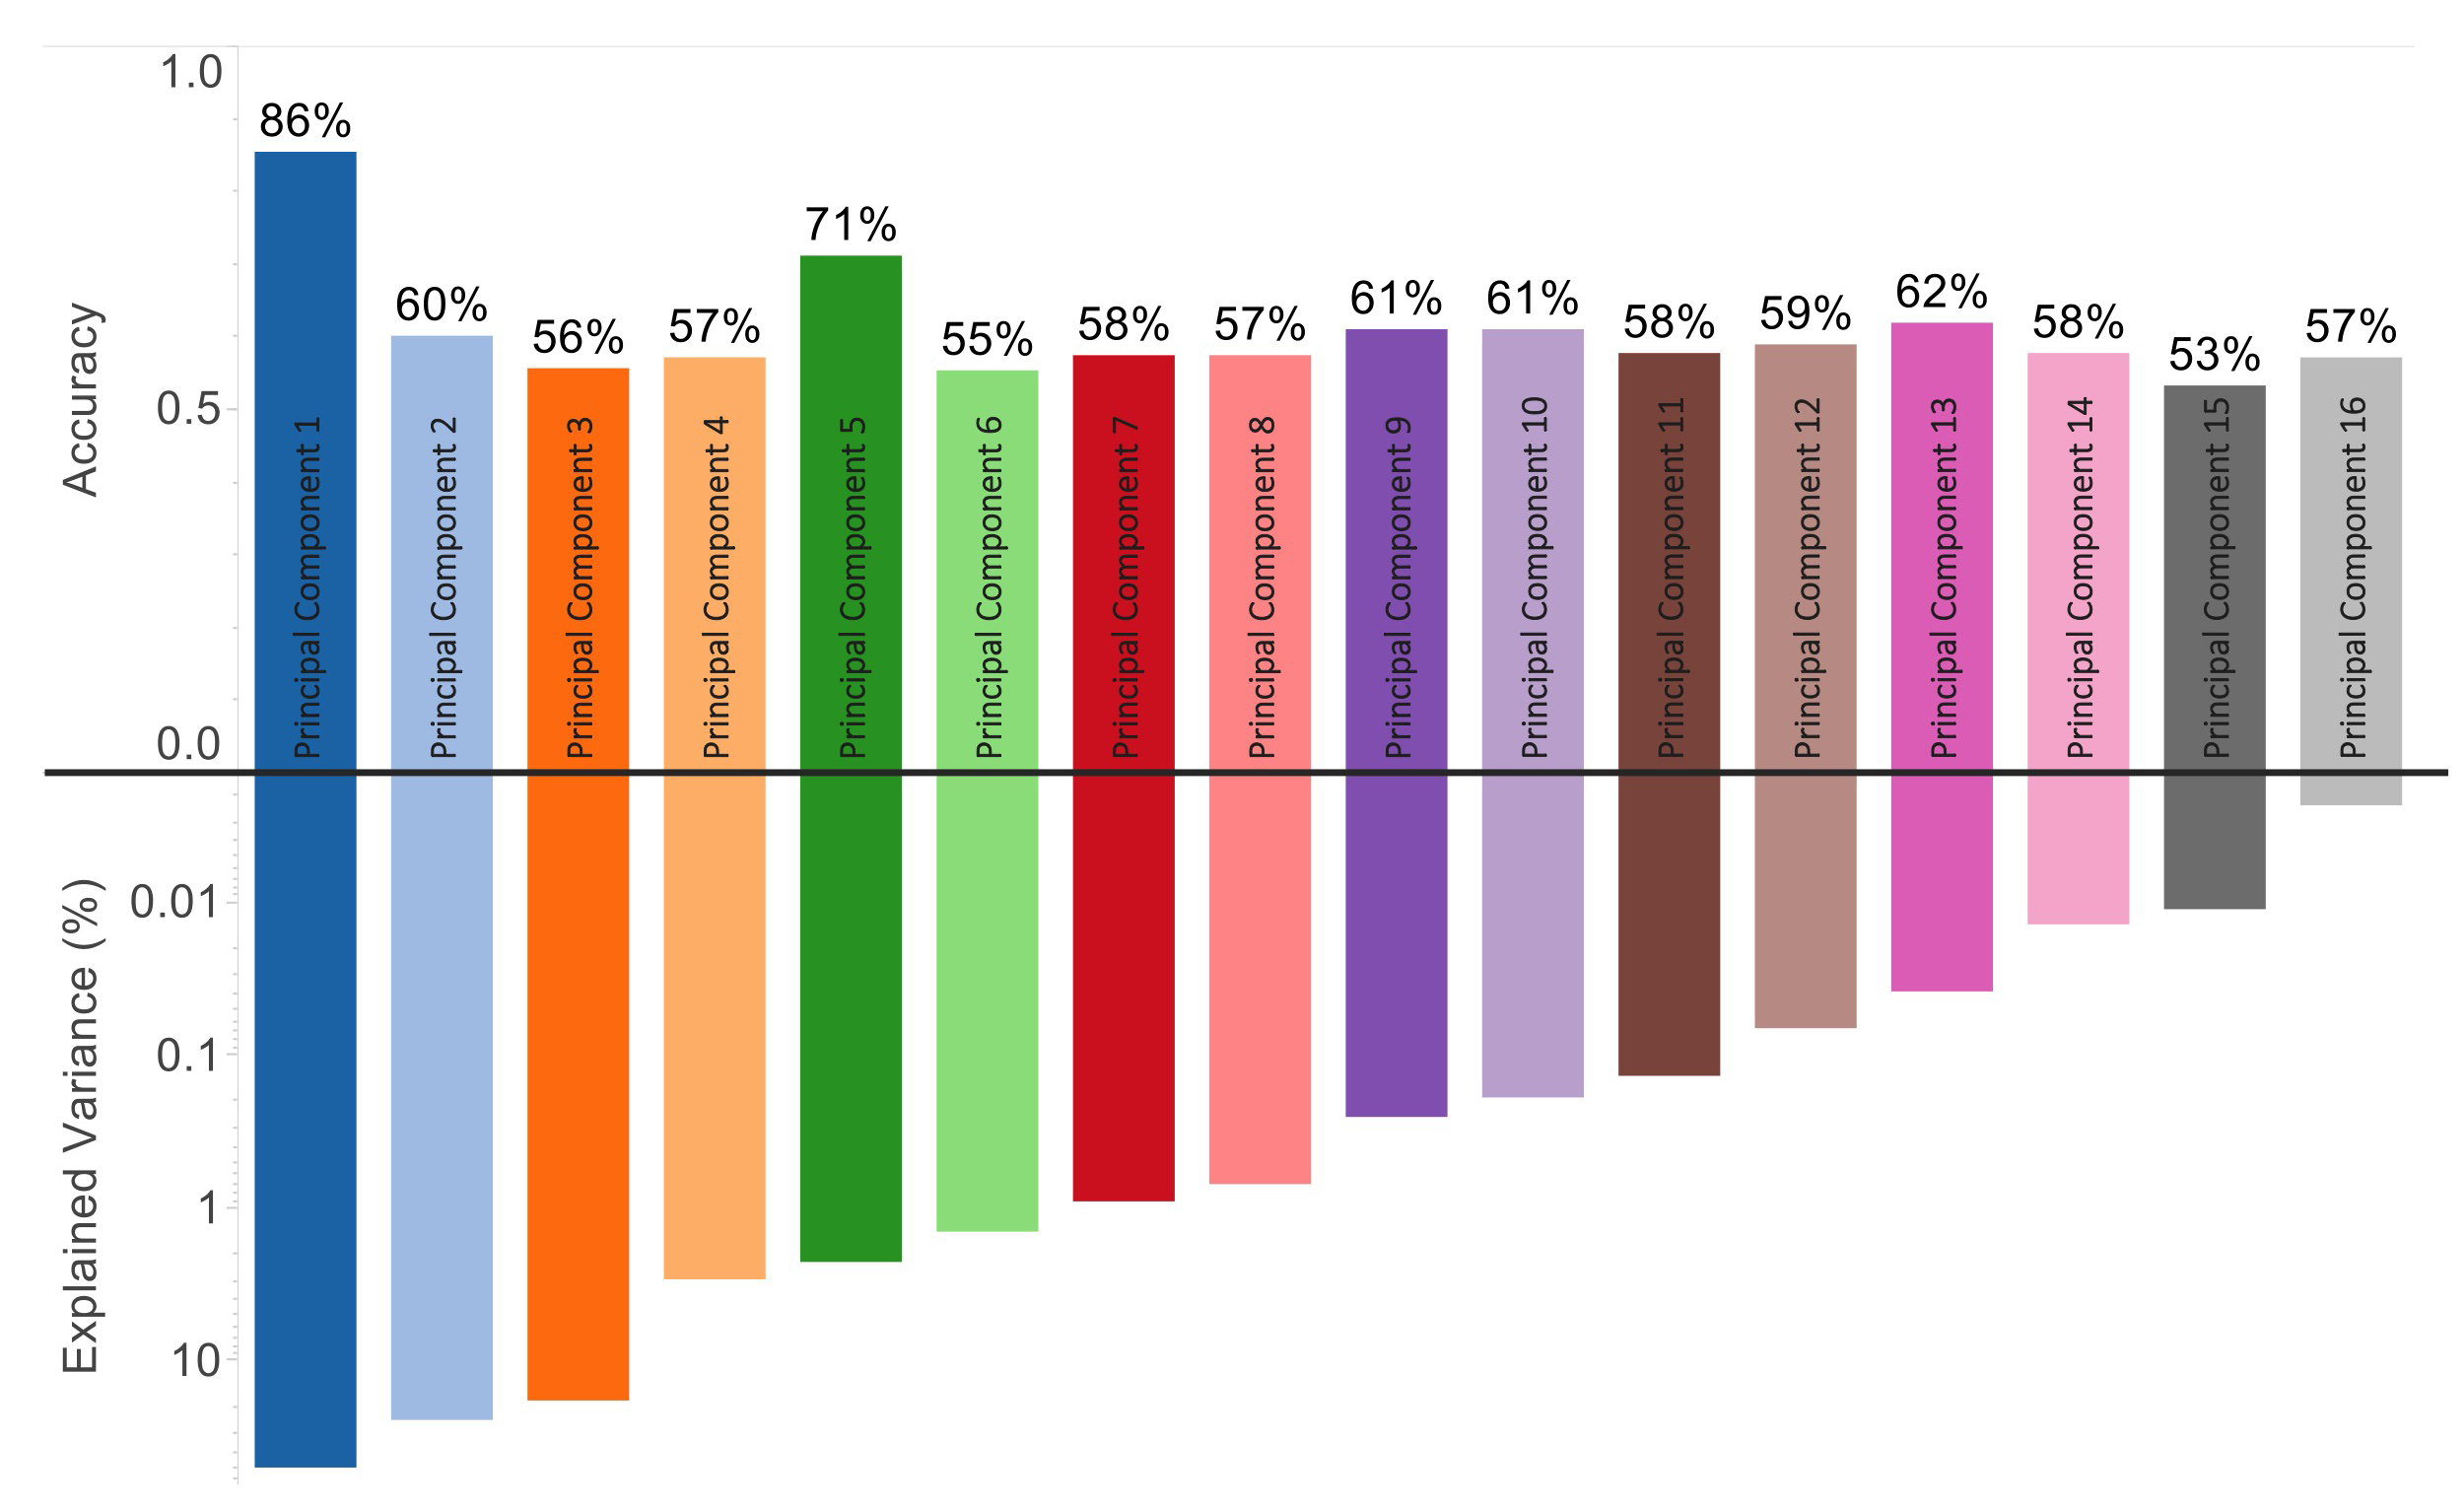
\includegraphics[scale=0.18]{FigurePCA.jpg}
\caption{\label{fig:PCA} Principal component analysis (PCA); Upper bar chart shows accuracy of classification by each individual principal component, and lower bar chart shows the percentage of the total variance explained by each principal component, accounting for the variability expressed in the data. As expected, principal components with larger variability do not necessarily give high accuracy in classification.}
\end{figure*}

\subsection{Regularization}

[] Regularization
[] Cross validation



[] 
\begin{figure}
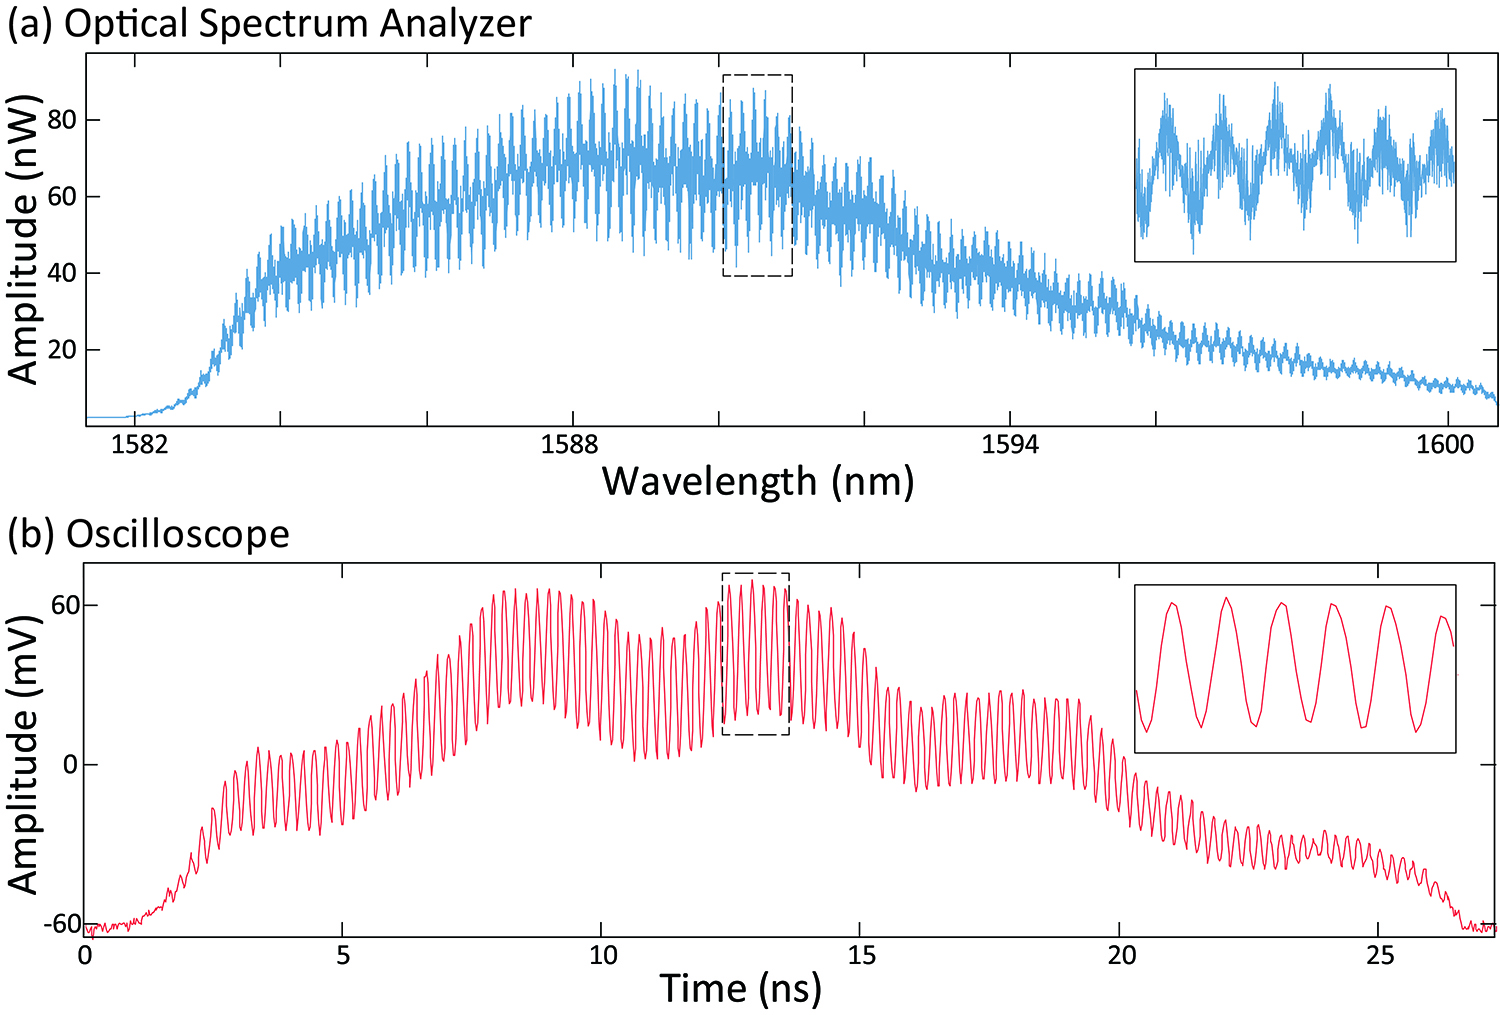
\includegraphics[scale=0.5]{FigureOSA.jpg}
\caption{\label{fig:OSA} Comparison of the interferograms measured by optical spectrum analyzer and time-stretch dispersive Fourier Transform; (a) Optical spectrum of the signal after quantitative phase imaging (box 1 in Fig.~\ref{fig:Setup}) and before it enters the amplified time-stretch system (box 2 in Fig.~\ref{fig:Setup}). The interference pattern in spectral domain is measured by an optical spectrum analyzer. (b) With time stretch, the interference pattern in spectral domain is linearly mapped into time. The baseband intensity envelope is slightly modified by the wavelength-dependent gain profile of the Raman amplifier. The inserts in panels a and b show the zoomed-in spectrum and waveform in the dashed black boxes, respectively. Clearly, the single-shot interferogram measured by Raman-amplified time-stretch dispersive Fourier Transform has a higher signal-to-noise ratio compared to that captured by optical spectrum analyzer.}
\end{figure}

\subsection{System performance and resolvable points}
Lateral resolution of time stretch camera is decided by the limiting factor among Abbe diffraction limit of the objective lens, spectral resolvability of the diffraction grating pairs, spectral resolution in amplified dispersive Fourier transform, the photodetector rise-time and bandwidth, and the sampling rate of the back-end digitizer. Details of the limiting factors of lateral resolution and evaluation of these factors for our TS-QPI system can be found in Table~\ref{tbl:Resolution}. Field of view (FOV) is the area covered by the interrogation rainbow when the rainbow pulses hit the imaging plane. The rainbow pulses width is decided by the optical bandwidth selected from the laser source, $\Delta\lambda$, the magnification factor of the objective lens as well as the focal length of the other lens and parabolic mirrors, and the dimensions and blaze angles of the diffraction gratings.

\begin{table*}
\caption{\label{tbl:Resolution} Resolution Limiting Factors in TS-QPI}
\begin{tabular}{|m{0.16\textwidth}|m{0.15\textwidth}|m{0.45\textwidth}|m{0.10\textwidth}|}
 \hline
 System catagory   &Component  &Number of resolvable points &Lateral resolution    \\  \hline
\multicolumn{1}{ |m{0.16\textwidth}  }{\multirow{2}{*}{Free-space optics} } &
\multicolumn{1}{ |m{0.15\textwidth}| }{Diffraction gratings} & \begin{equation} N_{grating} = \frac{\Delta\lambda}{\delta\lambda_{grating}} =\Delta\lambda /(\lambda \cdot \frac{d}{m\cdot2w_0})\end{equation} where $\Delta\lambda$ is the optical bandwidth, $\lambda$ is the central wavelength, m is the order of diffraction, $w_0$ is the beam waist, and $d$ is the groove spacing. &$\SI{3.09}{\micro\meter}$ \\ \cline{2-4}
\multicolumn{1}{ |m{0.15\textwidth}  }{}         &
\multicolumn{1}{ |m{0.15\textwidth}| }{Lenses and mirrors} & \begin{equation} N_{Abbe} = \frac{FOV}{\delta x_{diffraction}} =\frac{FOV}{(\frac{\lambda + \Delta \lambda/2}{2 \cdot NA})} \end{equation} where $FOV$ is field of view, $NA$ is numerical aperture of the objective lens. &$\SI{2.00}{\micro\meter}$   \\ \cline{1-4}
\multicolumn{1}{ |m{0.16\textwidth}  }{\multirow{1}{*}{Time Stretch} } &
\multicolumn{1}{ |m{0.15\textwidth}| }{Group delay dispersion} &\begin{equation}N_{DFT}=\frac{\Delta\lambda}{\delta\lambda}=\frac{\Delta\lambda}{\lambda\cdot\sqrt{\frac{2}{DL_f\cdot c}}}\end{equation} where $D$ is the group velocity dispersion, $L_f$ is the dispersive fiber length. &$\SI{0.73}{\micro\meter}$ \\ \cline{1-4}
\multicolumn{1}{ |m{0.16\textwidth}  }{\multirow{2}{*}{Electronic back-end} } &
\multicolumn{1}{ |m{0.15\textwidth}| }{Photodetector bandwidth} &\begin{equation}N_{PD}=\frac{\Delta t}{\delta t}=\frac{DL_f\Delta\lambda}{0.35/B}\end{equation} where $B$ is the bandwidth of the photodetector. &$\SI{0.28}{\micro\meter}$ \\ \cline{2-4}
\multicolumn{1}{ |m{0.15\textwidth}  }{} &
\multicolumn{1}{ |m{0.15\textwidth}| }{ADC sampling rate} &\begin{equation}N_{ADC}=DL_f\Delta\lambda f_{ADC}\end{equation} where $f_{ADC}$ is the sampling rate of digitizer. &$\SI{0.10}{\micro\meter}$ \\
\cline{1-4}
\end{tabular}
\end{table*}

The resolution of phase measurement along axial direction is determined by the effective number of bits (ENOB) of the digitizer and affected by the noise of laser source. Since pulse to pulse intensity and phase fluctuations are small, noise from laser source is not the limiting factor in our phase measurements. Supposing the ENOB of the digitizer is $N$, the minimum detectable optical path length difference, $\Delta L$ can be estimated as
\begin{equation}
\frac{1}{2}sin\left(\frac{4\pi \Delta L}{\lambda + \Delta \lambda/2}\right)=2^{-N}
\end{equation}
where $\lambda$ is the central wavelength of light, and $\Delta\lambda$ is the optical bandwidth. In our system, ENOB of the analog-to-digital converter is $5$. Thus, OPD resolution along the axial direction is about $\SI{8.0}{\nano\meter}$, corresponding to refractive index difference down to the order of $0.001$ for cellular level measurements.



\subsection{Microfluidic channel design and fabrication}

The Polydimethylsiloxane (PDMS) microfluidic channel is custom-designed so that it could fit into the reflective optics design. Cells are hydrodynamically focused \cite{knight1998hydrodynamic,lee2006hydrodynamic} at the center of the channel flowing at a velocity of 1.3 m/s. The microfluidic device consists of a hydrodynamic focusing region and an imaging region targeted by the interrogation rainbow flashes in TS-QPI system. At the hydrodynamic focusing region, the sheath pressure focused the sample at the center of the channel by narrowing its flow width from \SI{200}{\micro\meter} to about \SI{40}{\micro\meter} with a sheath to sample volume ratio of 3:1. The dimension of the channel was chosen as \SI{200}{\micro\meter} (width) $\times$ \SI{25}{\micro\meter} (height) so that the cells will be imaged within depth of view with a narrow lateral distribution. The size of the entire PDMS channel is optimized for fitting on a 2 inch diameter dielectric mirror with sufficient space at the edges to achieve strong bonding. The thickness of the channel top layer is optimized for stabilizing peek tubes performance reliability while accommodate the working distance of the objective lens. 

\begin{figure}[p]
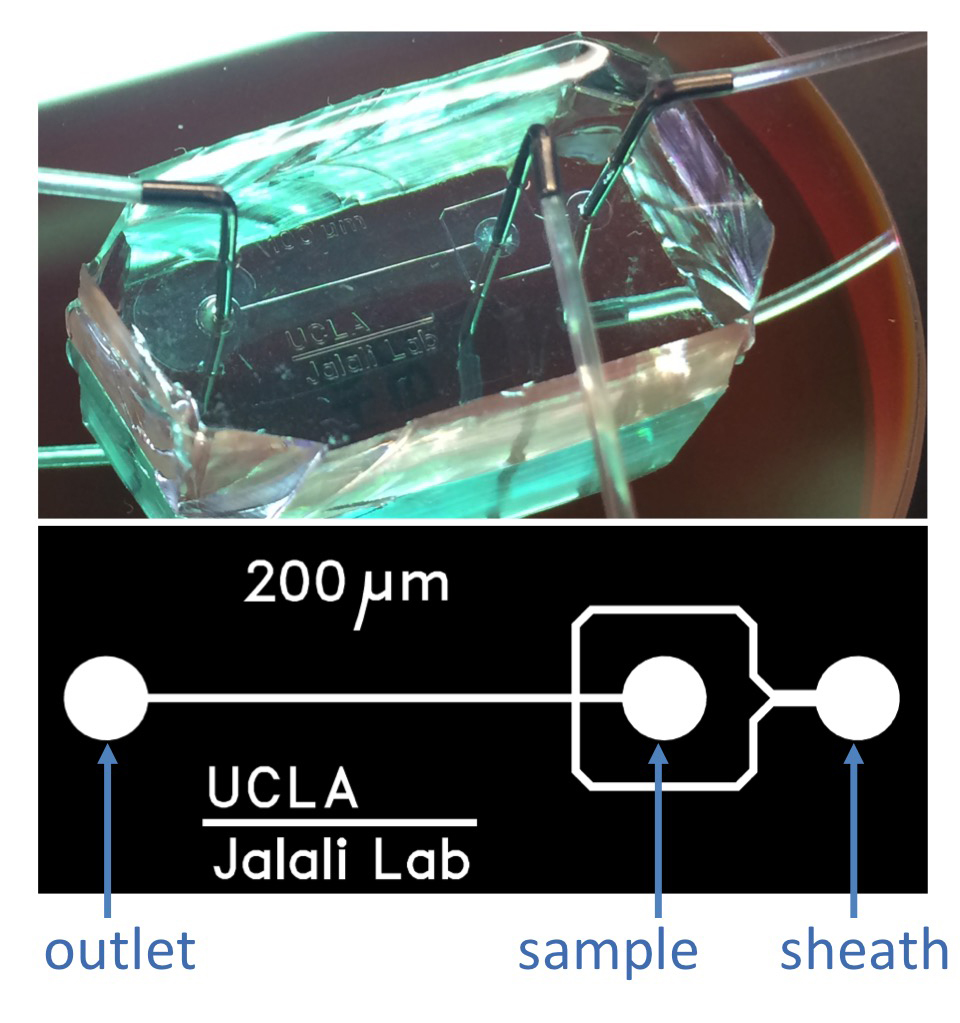
\includegraphics[scale=0.2]{FigureChannel.jpg}
\caption{\label{fig:Channel} PDMS microfluidic channel mounted on a highly reflective surface with near-infrared dielectric coating; The microfluidic device consists of a hydrodynamic focusing region and an imaging region targeted by the interrogation rainbow flashes in TS-QPI system. (a) Sample solution with suspended cells is fed into the channel through the sample inlet, and deionized water as the sheath flow is sent through sheath inlet. At the hydrodynamic focusing region, the sheath pressure focused the sample at the center of the channel by narrowing its flow width from \SI{200}{\micro\meter} to about \SI{40}{\micro\meter} with a sheath to sample volume ratio of 3:1. (b) The pattern of the mask used to imprint microfluidic channel design on silicon wafer with photoresist. The circles are inlet and outlet reservoirs.}
\end{figure}


The PDMS microfluidic channel (Fig.~\ref{fig:Channel}) is fabricated using standard soft lithography. The mask was designed in AutoCAD and printed with a resolution down to 1 um. Then a 4-inch silicon wafer was spin-coated with 75um thickness of a negative photoresist (SU-8 from MicroChem) and was exposured under the mask using an aligner. After post-exposure baking, the wafer was developed at room temperature, rinsed with isopropyl alcohol (IPA), and placed in a petri dish.  A PDMS mixture (Sylgard 184 Silicone Elastomer, Dow Corning) was poured onto the patterned wafer, degassed in a vacuum chamber for 30 min and cured at \SI{80}{\degreeCelsius} for one hour. Once cured, the PDMS channel was cut out and peeled off from the master wafer. We used 1.25 um diameter hollow needle to punch the inlet and outlet holes. 
The punched PDMS channel was then cleaned with nitrogen gun and magic tape (3M), treated with oxygen plasma (Enercon Dyne-A-Mite 3D Treater) for 2 min, and bonded to a 2-inch broadband dielectric mirror (Thorlabs BB2-E04) for obtaining high reflectance from channel substrate at near infrared spectral window. Finally microtubes (PE-50 tubing, .023x.038in) with steel catheter couplers (Instech, 22 ga x 15 mm) are connected to the inlet and outlet punctures.


\subsection{Preparation of algae cell lines}

\textit{Chlamydomonas reinhardtii} strains used were \textit{cw15} (\textit{nit1 NIT2 mt$^{+-}$}) and \textit{sta6} (\textit{cw15 nit1 NIT2 arg7-7 sta6-1::ARG7 mt$^+$}), available as CC-4568, CC-4348 respectively from the Chlamydomonas resource center (CRC)\cite{minnesota2015chlamydomonas}.

Cells were grown in tris-acetate-phosphate (TAP) medium supplemented with arginine (\SI{100}{\micro\gram\per\milli\liter}). Cultures were grown in Innova incubators (New Brunswick Scientific, Edison, NJ) at \SI{24}{\degreeCelsius}, agitated at 180 rpm with continuous light (\SI{95}{\micro\mole\per\square\meter\per\second}, 6 cool white fluorescent bulbs at \SI{4100}{\kelvin} and 3 warm white fluorescent bulbs at \SI{3000}{\kelvin} per incubator). To induce lipid production, cells were cultured to mid-log phase in regular TAP prior to deprivation of N by transfer to ammonium-free (i.e. nitrogen-free) TAP medium, as described previously \cite{blaby2013systems}. Briefly, cells subjected to nitrogen deprivation were grown to \SI{4e6}{\cells\per\milli\liter} and collected by centrifugation at 1006 xg for 5 min at room temperature. The supernatant was discarded, and the cells were washed in nitrogen-free TAP. Cells were then resuspended in nitrogen-free TAP to a final cell count of \SI{2e6}{\cells\per\milli\liter}. Cell densities were determined using a hemocytometer.


% Create the reference section using BibTeX:
%merlin.mbs apsrev4-1.bst 2010-07-25 4.21a (PWD, AO, DPC) hacked
%Control: key (0)
%Control: author (0) dotless jnrlst
%Control: editor formatted (1) identically to author
%Control: production of article title (0) allowed
%Control: page (1) range
%Control: year (0) verbatim
%Control: production of eprint (0) enabled
\begin{thebibliography}{4}%
\makeatletter
\providecommand \@ifxundefined [1]{%
 \@ifx{#1\undefined}
}%
\providecommand \@ifnum [1]{%
 \ifnum #1\expandafter \@firstoftwo
 \else \expandafter \@secondoftwo
 \fi
}%
\providecommand \@ifx [1]{%
 \ifx #1\expandafter \@firstoftwo
 \else \expandafter \@secondoftwo
 \fi
}%
\providecommand \natexlab [1]{#1}%
\providecommand \enquote  [1]{``#1''}%
\providecommand \bibnamefont  [1]{#1}%
\providecommand \bibfnamefont [1]{#1}%
\providecommand \citenamefont [1]{#1}%
\providecommand \href@noop [0]{\@secondoftwo}%
\providecommand \href [0]{\begingroup \@sanitize@url \@href}%
\providecommand \@href[1]{\@@startlink{#1}\@@href}%
\providecommand \@@href[1]{\endgroup#1\@@endlink}%
\providecommand \@sanitize@url [0]{\catcode `\\12\catcode `\$12\catcode
  `\&12\catcode `\#12\catcode `\^12\catcode `\_12\catcode `\%12\relax}%
\providecommand \@@startlink[1]{}%
\providecommand \@@endlink[0]{}%
\providecommand \url  [0]{\begingroup\@sanitize@url \@url }%
\providecommand \@url [1]{\endgroup\@href {#1}{\urlprefix }}%
\providecommand \urlprefix  [0]{URL }%
\providecommand \Eprint [0]{\href }%
\providecommand \doibase [0]{http://dx.doi.org/}%
\providecommand \selectlanguage [0]{\@gobble}%
\providecommand \bibinfo  [0]{\@secondoftwo}%
\providecommand \bibfield  [0]{\@secondoftwo}%
\providecommand \translation [1]{[#1]}%
\providecommand \BibitemOpen [0]{}%
\providecommand \bibitemStop [0]{}%
\providecommand \bibitemNoStop [0]{.\EOS\space}%
\providecommand \EOS [0]{\spacefactor3000\relax}%
\providecommand \BibitemShut  [1]{\csname bibitem#1\endcsname}%
\let\auto@bib@innerbib\@empty
%</preamble>
\bibitem [{\citenamefont {Knight}\ \emph {et~al.}(1998)\citenamefont {Knight},
  \citenamefont {Vishwanath}, \citenamefont {Brody},\ and\ \citenamefont
  {Austin}}]{knight1998hydrodynamic}%
  \BibitemOpen
  \bibfield  {author} {\bibinfo {author} {\bibfnamefont {James~B}\ \bibnamefont
  {Knight}}, \bibinfo {author} {\bibfnamefont {Ashvin}\ \bibnamefont
  {Vishwanath}}, \bibinfo {author} {\bibfnamefont {James~P}\ \bibnamefont
  {Brody}}, \ and\ \bibinfo {author} {\bibfnamefont {Robert~H}\ \bibnamefont
  {Austin}},\ }\bibfield  {title} {\enquote {\bibinfo {title} {Hydrodynamic
  focusing on a silicon chip: mixing nanoliters in microseconds},}\ }\href@noop
  {} {\bibfield  {journal} {\bibinfo  {journal} {Physical Review Letters}\
  }\textbf {\bibinfo {volume} {80}},\ \bibinfo {pages} {3863} (\bibinfo {year}
  {1998})}\BibitemShut {NoStop}%
\bibitem [{\citenamefont {Lee}\ \emph {et~al.}(2006)\citenamefont {Lee},
  \citenamefont {Chang}, \citenamefont {Huang},\ and\ \citenamefont
  {Yang}}]{lee2006hydrodynamic}%
  \BibitemOpen
  \bibfield  {author} {\bibinfo {author} {\bibfnamefont {Gwo-Bin}\ \bibnamefont
  {Lee}}, \bibinfo {author} {\bibfnamefont {Chih-Chang}\ \bibnamefont {Chang}},
  \bibinfo {author} {\bibfnamefont {Sung-Bin}\ \bibnamefont {Huang}}, \ and\
  \bibinfo {author} {\bibfnamefont {Ruey-Jen}\ \bibnamefont {Yang}},\
  }\bibfield  {title} {\enquote {\bibinfo {title} {The hydrodynamic focusing
  effect inside rectangular microchannels},}\ }\href@noop {} {\bibfield
  {journal} {\bibinfo  {journal} {Journal of Micromechanics and
  Microengineering}\ }\textbf {\bibinfo {volume} {16}},\ \bibinfo {pages}
  {1024} (\bibinfo {year} {2006})}\BibitemShut {NoStop}%
\bibitem [{\citenamefont {Laudon}(Data of
  access:20/07/2015)}]{minnesota2015chlamydomonas}%
  \BibitemOpen
  \bibfield  {author} {\bibinfo {author} {\bibfnamefont {Matt}\ \bibnamefont
  {Laudon}},\ }\href@noop {} {\enquote {\bibinfo {title} {Chlamydomonas
  resource center, university of minnesota},}\ }\bibinfo {howpublished}
  {\url{http://chlamycollection.org/}} (\bibinfo {year} {Data of
  access:20/07/2015}),\ \bibinfo {note} {online}\BibitemShut {NoStop}%
\bibitem [{\citenamefont {Blaby}\ \emph {et~al.}(2013)\citenamefont {Blaby},
  \citenamefont {Glaesener}, \citenamefont {Mettler}, \citenamefont
  {Fitz-Gibbon}, \citenamefont {Gallaher}, \citenamefont {Liu}, \citenamefont
  {Boyle}, \citenamefont {Kropat}, \citenamefont {Stitt}, \citenamefont
  {Johnson} \emph {et~al.}}]{blaby2013systems}%
  \BibitemOpen
  \bibfield  {author} {\bibinfo {author} {\bibfnamefont {Ian~K}\ \bibnamefont
  {Blaby}}, \bibinfo {author} {\bibfnamefont {Anne~G}\ \bibnamefont
  {Glaesener}}, \bibinfo {author} {\bibfnamefont {Tabea}\ \bibnamefont
  {Mettler}}, \bibinfo {author} {\bibfnamefont {Sorel~T}\ \bibnamefont
  {Fitz-Gibbon}}, \bibinfo {author} {\bibfnamefont {Sean~D}\ \bibnamefont
  {Gallaher}}, \bibinfo {author} {\bibfnamefont {Bensheng}\ \bibnamefont
  {Liu}}, \bibinfo {author} {\bibfnamefont {Nanette~R}\ \bibnamefont {Boyle}},
  \bibinfo {author} {\bibfnamefont {Janette}\ \bibnamefont {Kropat}}, \bibinfo
  {author} {\bibfnamefont {Mark}\ \bibnamefont {Stitt}}, \bibinfo {author}
  {\bibfnamefont {Shannon}\ \bibnamefont {Johnson}},  \emph {et~al.},\
  }\bibfield  {title} {\enquote {\bibinfo {title} {Systems-level analysis of
  nitrogen starvation--induced modifications of carbon metabolism in a
  chlamydomonas reinhardtii starchless mutant},}\ }\href@noop {} {\bibfield
  {journal} {\bibinfo  {journal} {The Plant Cell Online}\ }\textbf {\bibinfo
  {volume} {25}},\ \bibinfo {pages} {4305--4323} (\bibinfo {year}
  {2013})}\BibitemShut {NoStop}%
\end{thebibliography}%


\end{document}
%
% ****** End of file apstemplate.tex ******

